
%(BEGIN_QUESTION)
% Copyright 2008, Tony R. Kuphaldt, released under the Creative Commons Attribution License (v 1.0)
% This means you may do almost anything with this work of mine, so long as you give me proper credit

When two gears mesh, the teeth of one gear are able to apply a force ($F$) to the teeth of the other gear.  This force is the quotient of torque (twisting force, $\tau$) and gear radius ($r$), calculated the same for either gear:

$$\includegraphics[width=15.5cm]{i03296x01.eps}$$

$$F = {\tau_1 \over r_1}$$

$$F = {\tau_2 \over r_2}$$

\vskip 30pt

Knowing that the amount of force ($F$) will be the same for both gears, combine these two equations to arrive at a new equation solving for the second torque ($\tau_2$) in terms of the first torque ($\tau_1$) and the two radii ($r_1$ and $r_2$).  Be sure to show all your work!

\vskip 50pt

$\tau_2 =$

\vfil 

\underbar{file i03296}
\eject
%(END_QUESTION)





%(BEGIN_ANSWER)

This is a graded question -- no answers or hints given!

%(END_ANSWER)





%(BEGIN_NOTES)

$$\tau_2 = {r_2 \over r_1} \tau_1$$

%INDEX% Mathematics review: manipulating and combining equations to form a new equation

%(END_NOTES)


